\chapter{Syntax of Propositional Logic}

\section{Propositional Languages}

	\begin{enumerate}[\thesection.1]
	
		\item As we said in the introduction, formal languages are the result of abstracting away from the logically irrelevant aspects of ordinary language to arrive at an abstract, mathematical language with well-defined symbols and grammatical rules.  We also mentioned in the introduction that propositional logic is the logic of `not,' `and,' `or,' `if \dots, then \dots,' and `iff'---the so-called \emph{sentential operators}. Correspondingly, to define formal languages for propositional logic, we abstract away from everything but the structure required for the sentential operators. 
		
		\item What is this structure? ---First, note that the sentential operators connect sentences to form new sentences. The operator `not,' for example, takes a sentence and makes a new one out of it, it takes us from ``two plus two equals four'' to ``two plus two doesn't equal four.'' The operator `and,' instead takes two sentences to form a new one; from ``two plus two equals four'' and ``four is even,'' we get to ``two plus two equals four and four is even.'' Next, note that for validity in propositional logic, it actually doesn't matter what the sentences are that an operator connects. Take, for example, inference (1) from the introduction:
		\begin{enumerate}[(1)]
		
			\item The letter is either in the left drawer or in the right drawer, and it's not in the left drawer. So, the letter is in the right drawer.
		
		\end{enumerate}
This inference remains valid if we replace 	``the letter is in the left drawer'' and ``the letter is in the right drawer'' with any statements we please. The following inference, for example, is equally valid:	
		\begin{enumerate}[(1')]
		
			\item The cat is either on the mat or the dog dances tango, and the cat isn't on the mat. So, the dog dances tango.
		
		\end{enumerate}
To see this, just go through the reasoning we used to see that (1) is valid and replace ``the letter is in the left drawer'' everywhere with ``the cat is on the mat'' and ``the letter is in the right drawer'' with ``the dog dances tango.'' 

\item So, we can abstract away from the concrete sentences in an inference, and replace them with \emph{sentence letters}, typically written $p,q,r,\mathellipsis.$ The sentential operators, then, are represented by the following formal symbols: 
		\begin{center}
			\begin{tabular}{c | c | c}
			Symbol & Name & Reading\\ \hline
			
			$\neg$ & Negation & not\\
			$\land$ & Conjunction & and\\
			$\lor$ & Disjunction & or\\
			$\to$ & Conditional & if \dots, then \dots\\
			$\leftrightarrow$ & Biconditional & iff
			\end{tabular}
		\end{center}
So, the sentence ``the letter is either in the left drawer or in the right drawer'' becomes the formula $(p\lor q)$ and the sentence ``the letter is not in the left drawer'' becomes $\neg p$. If we use the symbol $\therefore$ to stand for the natural language expression ``so,'' we can therefore fully formally represent the inference (1) as:
 	\[(p\lor q),\neg p\therefore q\]
The abstraction process just described is the translation from natural language into the  language of propositional logic, which is known as \emph{formalization}. We will now first define the notion of a propositional language, a formal language of propositional logic, and then discuss how to formalize natural language claims in a propositional language.

		\item To define formal language (in propositional logic and beyond) we need to do two things: we need to specify a \emph{vocabulary}---the symbols we can use to form expression of the language---and we need to define a \emph{grammar}, which tells us which expressions of the symbols from the vocabulary are \emph{well-formed}.
		
		\item For a propositional language, typically denoted $\mathcal{L}$, the vocabulary consists of the following:		
		\begin{enumerate}[(i)]
		
			\item a (non-empty) set $\mathcal{P}$ of sentence letters,\footnote{In the following, we'll always assume that $\mathcal{P}$ only contains lower case letters $p,q,r, \mathellipsis$ and, in particular that $\neg,\land,\lor,\to,\leftrightarrow,(,)\notin\mathcal{P}$.}
			
			\item the \emph{sentential operators} $\neg,\land,\lor,\to,$ and $\leftrightarrow$, and 
			
			\item the \emph{parentheses} $($ and $)$.
		
		\end{enumerate}
		Every expression in $\mathcal{L}$ is constructed from the symbols in its vocabulary.
		
		\item The grammar of $\mathcal{L}$, then, is given by an inductive definition: we inductively define the set of well-formed formulas, typically denoted (somewhat ambiguously) simply $\mathcal{L}$. Remember that in order to recursively define a set, we need to give a set of initial elements and a set of constructions to form new elements from old ones. Well, in the case of a propositional language, the initial elements are simply the sentence letters and the constructions are given by the sentential operators. So, the set of well-formed formulas of $\mathcal{L}$ is defined as the smallest set $X$, such that:
		\begin{enumerate}[(i)]
		
			\item $\mathcal{P}\subseteq X$
			
			\item \begin{enumerate}[(a)]

					\item if $\phi\in X$, then $\neg \phi\in X$
					
					\item if $\phi,\psi\in X$, then $(\phi\land\psi), (\phi\lor\psi),(\phi\to\psi),(\phi\leftrightarrow\psi)\in X$.
		
				\end{enumerate}		
		
		\end{enumerate}
Note the presence of the parentheses in (ii.b)---we'll have to talk about them in some more detail later. It's a bit tedious to write out (ii.b) in full, so we sometimes use the following notation, in which $\circ$ is a variable ranging over the sentential connectives:
\begin{enumerate}[(i)]
		\setcounter{enumii}{1}
			
			\item \begin{enumerate}[(a)]
		\setcounter{enumiii}{1}
					
					\item if $\phi,\psi\in X$, then $(\phi\circ\psi)\in X$, for $\circ=\land,\lor,\to,\leftrightarrow$.
		
				\end{enumerate}		
		
		\end{enumerate}
So, for example, if $\mathcal{P}$ is the set $\{p,q,r\}$, we have $p, \neg\neg q, (p\land (r\lor q)), (p\to (r\lor (p\land (q\leftrightarrow r)))), \mathellipsis\in\mathcal{L}$.	

	\item Note that there are many different propositional languages, one for each set of propositional letters. For example, the language defined over $\mathcal{P}=\{p\}$ is different from the language defined over $\mathcal{P}=\{p,q\}$. The latter, for example, contains $(p\land q)$ as a formula, while the former does not. In the following, we'll always assume that we're dealing with a fixed propositional language $\mathcal{L}$, which has $p,q,r,\mathellipsis\in\mathcal{P}$.

	\item There is another way of writing the grammar of a propositional language, which you should have seen. This is the so-called \emph{Backus-Naur-Form} or \emph{BNF}, for short, which is especially important in programming and computer science. The BNF of a propositional language is given as follows:
	\[\phi::=p~|~\neg \phi~|~(\phi\land\phi)~|~(\phi\lor\phi)~|~(\phi\to\phi)~|~(\phi\leftrightarrow\phi)\]
This BNF means precisely the same thing as our official recursive definition, it is just written differently. The idea is that an object of type $\phi$ (formula) is either a sentence letter, $p\in\mathcal{P}$, the result of taking an object of type $\phi$ and writing a $\neg$ in front of it, or the result of taking an object of type $\phi$ another object of type $\phi$ and writing a sentential operator between the two and packaging the result in parentheses.
	
	\item With the official definition of $\mathcal{L}$ in place, we can straight-forwardly show that an expression is a formula by constructing it from the sentence letters using the sentential operators. For example, we can show that $(p\land (q\lor r))\in\mathcal{L}$ (assuming that $p,q,r\in\mathcal{P}$) as follows :
	\begin{itemize}
	
		\item We have $q,r\in\mathcal{P}$, therefore $q,r\in\mathcal{L}$.
		
		\item Since $q,r\in\mathcal{L}$, we have that $(q\lor r)\in\mathcal{L}$.
		
		\item We have $p\in\mathcal{P}$ and therefore $p\in\mathcal{L}$.
		
		\item Since $(q\lor r), p\in\mathcal{L}$, we get that $(p\land (q\lor r))\in\mathcal{L}$.
	
	\end{itemize} 
And we can also show that an expression is not a formula, roughly like we showed that something is not a natural number. Here, as an example, we'll show that $(p\land\neg)\notin\mathcal{L}$ (even if $p\in\mathcal{P}$):

	\begin{proposition}
	Let $\mathcal{L}$ be a propositional language. Then $(p\land \neg)\notin\mathcal{L}$.
	\end{proposition}
	\begin{proof}
	Let $X$ be a set such that $X$ satisfies conditions (i) and (ii) from the definition of $\mathcal{L}$ and $(p\land \neg)\in X$. We claim that then the set $Y$ defined by: \[Y=X\setminus \{(p\land \neg), \neg\}\] also satisfies conditions (i) and (ii) and $Y\subset X$. We need to show two things. First, we show that (i) $\mathcal{P}\subseteq Y$. To see this, note that $\mathcal{P}\subseteq X$ and $(p\land \neg), \neg\notin\mathcal{P}$. So it follows that for all $p\in\mathcal{P}$, $p\in X$ and $p\notin  \{(p\land \neg), \neg\}$. Hence, $p\in Y$, meaning $\mathcal{P}\subseteq Y$.
	
	To see that $Y$ satisfies condition (ii.a), let's suppose that $\phi\in Y$. Since $Y= X\setminus \{(p\land \neg), \neg\}$, it follows that $\phi\in X$. And since $X$ is closed under negation, we can conclude that $\neg\phi\in X$. But clearly $\neg \phi\notin \{(p\land \neg), \neg\}$. Hence, $\phi\in X\setminus  \{(p\land \neg), \neg\}$, meaning $\phi\in Y$.
	
	To see that $Y$ satisfies condition (ii.b), assume that $\phi,\psi\in Y$. We now need to show four different cases (a) $(\phi\land\psi)\in Y$, (b) $(\phi\lor\psi)\in Y$, (c) $(\phi\to\psi)\in Y$, and (d) $(\phi\leftrightarrow\psi)\in Y$. But for cases (b--d), this is easy. Since $\phi,\psi\in Y$, we get that $\phi,\psi\in X$. Since $X$ satisfies (ii.b), we get that $(\phi\circ\psi)\in X$ for $\circ=\lor,\to,\leftrightarrow$. And trivially, for  $\circ=\lor,\to,\leftrightarrow$, $(\phi\circ\psi)\notin \{(p\land \neg), \neg\}$. Hence $(\phi\circ\psi)\in Y$, as desired. (Why trivially? We'll look at the form of the members of $\{(p\land \neg), \neg\}$\dots)
	
	Only in case (a), we need to reason a bit more. We again easily get from $\phi,\psi\in Y$ to $\phi,\psi\in X$ and from there via (ii.b) to $(\phi\land\psi)\in X$. But can $(\phi\land\psi)$ be in $\{(p\land \neg), \neg\}$? Well, only if $\phi=p$ and $\psi=\neg$. But remember that $\psi\in Y=X\setminus \{(p\land \neg), \neg\}$. Hence if $\psi=\neg$, then $\psi\notin Y$, which contradicts our assumption that $\psi\in Y$. Hence, using proof by contradiction, we can conclude that $(\phi\land\psi)\notin\{(p\land \neg), \neg\}$. Hence $(\phi\land\psi)\in Y$, as desired.
	
	So, if $X$ satisfies (i) and (ii) and $(p\land \neg)\in X$, then $X$ is not the smallest set that satisfies conditions (i) and (ii). Hence $X\neq \mathcal{L}$. For a final proof by contradiction, suppose that $(p\land \neg)\in\mathcal{L}$. By our observation, it would follow that $\mathcal{L}\neq\mathcal{L}$, which is a contradiction. Hence $(p\land \neg)\notin\mathcal{L}$.
	
	\end{proof}
	
	As you can see, it's quite tedious to show that something isn't a formula. In the following, we'll develop some techniques for proving that expressions aren't formulas that are a bit more ``user friendly.''
		
	\item But first, let's talk about formalization. As we said above, formalization is the process of abstracting a natural language expression into an expression of a formal language. We don't do this just for fun (even though it is fun), but with a particular aim in mind: we want to check inferences couched in natural language for validity. How to actually check for validity will be covered in the following chapter. For now you can note that in order for us to be able to draw any conclusion from our formal language expeditions back to ordinary language, we need to make sure that, whatever we do in our formalization, we can always reverse it---we want to be able to ``translate backwards.'' In order to guarantee this, every formalization begins with a \emph{translation key}, which is basically like a cipher in cryptography. A translation key tells us for each sentence letter which natural language sentence it stands for. 
	
Here's an example of a translation key:
	\begin{center}
	\begin{tabular}{c c c}
	$p$ & : & the letter is in the left drawer\\
	$q$ & : & the letter is in the right drawer
	\end{tabular}
	\end{center}
This is just one possible key, the following one is also perfectly fine:
	\begin{center}
	\begin{tabular}{c c c}
	$p$ & : & the letter is in the right drawer\\
	$q$ & : & the letter is in the left drawer
	\end{tabular}
	\end{center}	
The only thing you're not allowed to do in your translation key is to use a sentence letter to stand for an expression that is formed from simpler sentences using sentential connectives. So the following key is \emph{not} valid:
	\begin{center}
	\begin{tabular}{c c c}
	$p$ & : & the letter is in the left drawer\\
	$q$ & : & the letter is in the right drawer\\
	$r$ & : & the letter is not in the left drawer
	\end{tabular}
	\end{center}
Note that if a sentence is not directly formed from simpler sentences using the connectives, it is also translated by a sentence letter. For example, the sentence ``necessarily, it's not the case that humans fly'' get's translated as a sentence letter. Otherwise, there is no such thing as a correct key, only a useful one.

\item The rest of the process of formalization in propositional logic basically consists in finding the sentence operator that corresponds best to the operators used to form the sentence. There are no clear rules for doing so, but I can give you some guidelines. In the following examples, I use the translation key:
	\begin{center}
	\begin{tabular}{c c c}
	$p$ & : & the letter is in the left drawer\\
	$q$ & : & the letter is in the right drawer
	\end{tabular}
	\end{center}
Here are some simple sentences and their corresponding translations:	\begin{longtable}{p{8cm} c c}
	The letter isn't in the left drawer & $\leadsto$ & $\neg p$\\[1ex]
	It's not the case that the letter is in the left drawer & $\leadsto$ & $\neg p$\\[1ex]
	The letter is in the left and in the right drawer & $\leadsto$ & $(p\land q)$\\[1ex]
	The letter is not in the left drawer, but it's also not in the right one & $\leadsto$ & $(\neg p\land \neg q)$\\[1ex]
	The letter is in the left or in the right drawer & $\leadsto$ & $(p\lor q)$\\[1ex]
	The letter is neither in the left nor in the right drawer  & $\leadsto$ & $(\neg p\land \neg q)$\\[1ex]
	If the letter is in the left drawer, then it's not in the right drawer & $\leadsto$ & $(p\to \neg q)$\\[1ex]
	The letter is in the left drawer, if it's not in the right one & $\leadsto$ & $(\neg q\to p)$\\[1ex]
	The letter is only in the left drawer, if it's not in the right one & $\leadsto$ & $(p\to \neg q)$\\[1ex]
	The letter is in the left drawer iff it's not in the right one & $\leadsto$ & $(p\leftrightarrow \neg q)$\\
	\end{longtable}
	As you can see, $\neg,\land,\lor,\to,\leftrightarrow$ are basically used like their natural language counterparts. There are some special cases, however. Note, for example, that ``The letter is not in the left drawer, but it's also not in the right one'' becomes $(\neg p\land \neg q)$. This is because, from the perspective or propositional logic, the ``but'' only carries the information that both sentences are true---the implicit sense of surprise implied by the use of ``but'' is something we don't care about from a logical perspective.
	
	\item A very special case is the one of ``either \dots or \dots.'' This expression is ambiguous in English between an inclusive reading (one of the two or both) and an exclusive reading (one of the two but not both). The inclusive reading is translated as $\lor$ (by logical convention). So, ``the letter is either in the left drawer or in the right drawer'' would be translated as $(p\lor q)$ if read inclusively. But in this case, an \emph{exclusive} reading seems more appropriate. This reading would be translated as $((p\lor q)\land \neg (p\land q))$. It's usually possible from the context to determine which reading is intended, but sometimes there is simply a remaining ambiguity in natural language.\footnote{Just check [dictionary].}
	
	\item To conclude our brief treatment of formalization, let me say that being able to provide a good formalization is much like translating well from one language to another. It requires a good understanding of both and a careful attention to linguistic subtlety. As such, formalization is something you'll have to learn, slowly. You'll be much better at it, once you've properly understood how formal languages work, what the meaning of formal expressions is, given by their semantics, and so on. For now, my advice is just: exercise, exercise, exercise.

	\end{enumerate}
	
\section{Proof by Induction on Formulas}

\emph{The following section contains the first treatment of one of the most important principles of this course: proof by induction on formulas. Our entire treatment of mathematical induction was in preparation for this. So, before you embark on this section, make sure that you got as much as possible from our treatment of mathematical induction in the previous chapter.}

	\begin{enumerate}[\thesection.1]

		\item We will now develop the technique of proof by induction on formulas, or as we'll often simply call it from now on ``proof by induction.'' The principle is essentially the same as for $\mathbb{N}$ or the gargles, just applied to the formulas of a propositional language. So, remember that induction is a method for proving something for all members of an inductively defined set. We do so by showing first that the claim holds for all initial elements of the set and that it's preserved under its constructions. Spelled out for formulas, this leads to the following induction principle:
		\begin{theorem}
		Let $\Phi$ be a condition on formulas. If we can show:
		\begin{enumerate}[(i)]
		
			\item For all $p\in\mathcal{P}$, $\Phi(p)$.
			
			\item \begin{enumerate}[(a)]
			
			\item For all $\phi\in\mathcal{L}$, if $\Phi(\phi)$, then $\Phi(\neg\phi)$.

			\item For all $\phi,\psi\in\mathcal{L}$, if $\Phi(\phi)$ and $\Phi(\psi)$, then $\Phi((\phi\circ\psi))$, for $\circ=\land,\lor,\to,\leftrightarrow$.
		
		\end{enumerate}
		\end{enumerate}
		Then we can conclude that for all $\phi\in\mathcal{L}$, $\Phi(\phi)$.
		\end{theorem}
		\begin{proof}
		Let $\Phi$ be an arbitrary condition on formulas satisfying conditions (i) and (ii), Consider the set $\{x:\Phi(x)\}$. By the conditions (i) and (ii) of our theorem, $\{x:\Phi(x)\}$ satisfies conditions (i) and (ii) from the definition of $\mathcal{L}$. Since $\mathcal{L}$ is the smallest set satisfying those conditions, we have that $\mathcal{L}\subseteq\{x:\Phi(x)\}$. But now, it easily follows that for all $\phi\in\mathcal{L}$, we have that $\Phi(\phi)$. For let $\phi\in\mathcal{L}$ be an arbitrary formula. Since $\mathcal{L}\subseteq\{x:\Phi(x)\}$, it follows that $\phi\in\{x:\Phi(x)\}$. But that just means that $\Phi(\phi)$, as desired.
		\end{proof}
		
		\item We're going to use induction on formulas \emph{a lot} in this course. Almost always when I ask you ``how are we going to prove this?,'' the answer is going to be ``by induction, of course!'' So, let's be clear on how you write a proof by induction:
			\begin{enumerate}[1.]
		
			\item State clearly that you're using induction to prove the claim.
			
			\item Prove the base case, i.e. show that all sentence letters have the property.
			
			\item State clearly that you're now considering the induction steps. In each sub-case, begin by stating your induction hypothesis and then use it to derive the claim about the constructed element, i.e.
			\begin{itemize}
			
				\item derive that $\neg\phi$ has the property from the induction hypothesis that $\phi$ has the property, and
				
				\item derive that $(\phi\circ\psi)$ has the property (for $\circ=\land,\lor,\to,\leftrightarrow$) from the induction hypotheses that $\phi$ and $\psi$ has the property.
			
			\end{itemize}
			
			\item State clearly that you're using induction to infer that the claim in question holds for all elements of the set.
		
		\end{enumerate}
		
	\item We're now going through some applications of induction on formulas---but not just for the sake of it, there's going to be a purpose. We want to establish some criteria for determining that an expression isn't a formula. 
	
	\item First, we're going to note a fact about parentheses, which essentially depends on the fact that for every opening parentheses, there has to be a corresponding closing one in a proper formula. The fact is the following:
	\begin{proposition}
	Let $\phi\in\mathcal{L}$ be a formula. Then $\phi$ contains an even number of parentheses.
	\end{proposition}
	\begin{proof}
	We prove this by induction on formulas. 
	
	\begin{itemize}
	
		\item \emph{Base case}. No sentence letter contains any parentheses. So for each $p\in\mathcal{P}$, the number of parentheses in $p$ is zero. But zero is an even number. So, the base case holds.
		
		\item \emph{Induction steps.}
		
		\begin{itemize}
		
			\item Suppose the induction hypothesis that $\phi\in\mathcal{L}$ contains an even number of parentheses. Consider the formula $\neg\phi$. Note the number of parentheses in $\neg\phi$ are exactly the same as in $\phi$, since no new ones have been added. So, also $\neg\phi$ contains an even number of parentheses, as desired.
			
			\item Suppose the induction hypothesis that $\phi,\psi\in\mathcal{L}$ contain an even number of parentheses. Consider the formulas $(\phi\circ\psi)$. The number of parentheses in $(\phi\circ\psi)$ are precisely the number of parentheses in $\phi$, plus the number of parentheses in $\psi$, plus two. But that's the sum of three even numbers, and as such (as you proved as an exercise in the previous chapter) even, as desired.
		
		\end{itemize}
	
	\end{itemize}
	
	We conclude by induction on formulas that for every $\phi\in\mathcal{L}$, the number of parentheses in $\phi$ is even.
	
	\end{proof}
	
	This proposition already gives us a useful criterion for formula-hood: if an expression contains an odd number of parentheses, it cannot be a formula.
	
	\begin{corollary}
	Let $\phi$ be an expression. If $\phi$ contains an odd number of parentheses, then $\phi\notin\mathcal{L}$.
	\end{corollary}
	\begin{proof}
	Immediate from the previous proposition via contrapositive proof.
	\end{proof}
	Using this result, we can show, for example, that $((\neg(p\lor q)\land (p\leftrightarrow\neg\neg s))\notin\mathcal{L}$. Proving this with our definitional technique (the technique from 4.1.9) would be \emph{tedious}. But is it the best we can do using parentheses? Why, no! You will prove an even sharper result as an exercise at the end of this chapter.
			
	\item Before we move to the next section, we will prove one more useful result for proving that something isn't a formula. Note that we said that every formula of $\mathcal{L}$ is made up of symbols from its vocabulary. It's high-time, we proved this:
	\begin{proposition}
	Let $\phi\in\mathcal{L}$ be a formula. Then $\phi$ only contains symbols from the vocabulary of $\mathcal{L}$.
	\end{proposition}	
		\begin{proof}
		We prove this, again, by induction.
		
		\begin{itemize}
	
		\item \emph{Base case}. All the members of $\mathcal{P}$ are part of the vocabulary of $\mathcal{L}$. So, the base case holds.
		
		\item \emph{Induction steps.}
		
		\begin{itemize}
		
			\item Suppose the induction hypothesis that $\phi\in\mathcal{L}$ only contains symbols from $\mathcal{L}$'s vocabulary. Consider the formula $\neg\phi$. Note the symbols in $\neg\phi$ are exactly the same as in $\phi$ with the sole addition of $\neg$. But $\neg$ is a symbol of $\mathcal{L}$'s vocabulary. So also $\neg\phi$ only contains symbols from $\mathcal{L}$'s vocabulary.
			
			\item Suppose the induction hypotheses that $\phi,\psi\in\mathcal{L}$ only contain symbols from $\mathcal{L}$'s vocabulary. Consider the formula $(\phi\circ\psi)$, for $\circ=\land,\lor,\to,\leftrightarrow$. Note the symbols in $(\phi\circ\psi)$ are exactly the same as in $\phi$ and $\psi$ with the  addition of $(,\circ,$ and $)$. But  $(,\circ,$ and $)$ are all symbols of $\mathcal{L}$'s vocabulary. So also $(\phi\circ\psi)$ only contains symbols from $\mathcal{L}$'s vocabulary.
		
		\end{itemize}
	
	\end{itemize}
	
	We conclude the theorem by the principle of induction on formulas.
		
		\end{proof}	
			
	Also this result leads to a necessary condition for formula-hood:
	
	\begin{corollary}
	Let $\phi$ be an expression. Then, if $\phi$ contains a symbol not from $\mathcal{L}$'s vocabulary, then $\phi\notin\mathcal{L}$.
	\end{corollary}
	\begin{proof}
	Immediate from the previous proposition via contrapositive reasoning.
	\end{proof}
	
	This criterion allows us to exclude a whole range of expressions from $\mathcal{L}$, such as, for example, $(p\leftrightarrow (q\to \neg\neg\clubsuit))$. Again, this could be done using our definition method (4.1.9) but it would be tedious. In the next section, as an off-shoot from an important theoretical concept to do with readability, we'll get our strongest criterion for formula-hood---an actual algorithm we can use to figure out whether an expression is a formula.
			
	\end{enumerate}

\section{Unique Readability and Parsing Trees}

	\begin{enumerate}[\thesection.1]

		\item Remember the issues of gargle-readability (3.7.14). The problem was that some gargle could be constructed in more than one ways, which lead to a problem with function recursion over the gargles. We won't run into the same problem with formulas, but that's a fundamental fact about them---the so-called \emph{unique readability theorem}. Essentially, the theorem states that for each formula, there is a unique way to construct that formula from the sentence letters using the sentential connectives. Importantly, this makes formal languages computer-readable: it means that a computer, who lacks human intuition and context-sensitivity, can always precisely figure out what a given formula is supposed to say.
		
		\item The unique readability theorem is, in effect, a consequence of our tidy use of parentheses. To illustrate how, consider the ``formula'' $p\land q\lor r$, which is of course not a proper formula, but suppose for a second that we would allow expressions like this. Well, there would be two ways of ``reading'' or \emph{parsing} that formula:
		
		\begin{center}
		
		\begin{tabular}{c c c}
		\begin{tikzpicture}
		{\Tree [.$p\land q\lor r$ [.$p$ ] [.$q\lor r$ [.$q$ ] [.$r$ ] ] ]}
		\end{tikzpicture}

		& 
		
		\qquad \raisebox{7.5ex}{vs.} \qquad 
				\begin{tikzpicture}

		{\Tree [.$p\land q\lor r$ [.$p\land q$ [.$p$ ] [.$q$ ] ] [.$r$ ] ]}
		\end{tikzpicture}

		\end{tabular}
		\end{center}
This is not only bad for function recursion (for issues we discussed in the context of the gargles) but also messes up our intended \emph{informal} reading of the formula. Suppose we use a translation key where $p$ stands for ``I drink a coffee,'' $q$ for ``I have toast,'' and $r$ for ``I have eggs.'' Then, our two ways of parsing the sentence correspond to two very different informal meanings:
	\begin{itemize}
	
		\item I have a coffee and either toast or eggs.
		
		\item Either I have a coffee and toast or I have eggs.
	
	\end{itemize}
The two are really very different in meaning: in the former case you have a beverage and food and in the second either you have a beverage and food or just some food.

But this is just a cautionary tale: the problem actually doesn't arise in propositional logic, as long as we use our parentheses properly---which is what we're going to prove in this section.

	\item To state the unique readability theorem, we will make use of the notion of a \emph{parsing tree}. And before that, the notion of a \emph{tree}.\footnote{Mathematicians call the structure that we're studying here (more correctly) a \emph{directed rooted} tree, but for simplicity we'll just drop the modifiers.} Roughly speaking, a tree is a structure of the following form:

\begin{center}
\begin{tikzpicture}
\Tree [.$\bullet$ [.$\bullet$  [.$\bullet$ {$\vdots$} {$\vdots$} ]  [.$\bullet$ {$\vdots$} ] ] [.$\bullet$  [.$\bullet$ [.$\bullet$ ] ]  [.$\bullet$ {$\vdots$} ]  [.$\bullet$ ] ] ]
\end{tikzpicture}
\end{center}

Some terminology about trees: 
	\begin{itemize}
		
		\item The dots are called the {\it nodes} of the tree and the lines connecting them the {\it edges}. 
		
		\item The upper-most node is called the {\it root} of the tree and the lower-most nodes its {\it leaves}. 
		
		\item If $x$ is a node in the tree and $y$ is directly above $x$, i.e. there is an edge pointing from $y$ to $x$, then $x$ is called a {\it child} of $y$ and $y$ the \emph{parent} of $x$. 
		
		\item A {\it path} in the tree is a sequence of nodes which are connected by edges. 
		
	\end{itemize}
Note that in a tree, there's never a ``loop,'' i.e. a (non-trivial) path that both begins and ends at the same node. We're not going to bother giving a mathematically precise definition of a tree, but instead we're going to put the concept immediately to (good) use.

	\item To define the parsing tree of a formula, we will, for the first time, make use of function recursion over $\mathcal{L}$. So let's briefly remind ourselves how this works in general (remember 3.7.12--13). In order to recursively define a function over an inductively defined set:
	
	\begin{enumerate}[1.]
		
			\item We say what the value of our function is on the initial elements.
			
			\item We say how to calculate the value of the function for an element built by a construction, where we can reference to the values of the function for the elements the element is constructed from.
		
		\end{enumerate}
	In the case of $\mathcal{L}$, this means we have to give the values of the function for all sentence letters and we have to say how the function behaves under the sentential operators. Note that we will have to prove that this actually defines a function on $\mathcal{L}$---remember the unique readability issue. We'll do in a moment. For now, we will pretend that it does and justify that assumption \emph{ex post}, i.e. afterwards.
	
	\item We will now use function recursion to define a function $T$, which maps any formula $\phi\in\mathcal{L}$ to its parsing tree:
	
\begin{center}
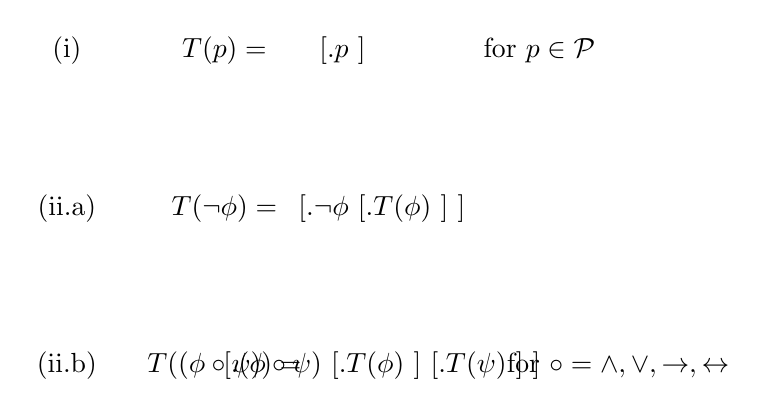
\begin{tikzpicture}
\node at (-2,1) {(i)};

\node at (0,1) {$T(p)=$};
\node at (1.5,1) {\Tree [.$p$ ]};
\node at (4,1) {for $p\in\mathcal{P}$};

\node at (-2,-1) {(ii.a)};
\node at (0,-1) {$T(\neg \phi)=$};
\node at (2,-1) {\Tree [.$\neg \phi$ [.$T(\phi)$ ] ]};

\node at (-2,-3) {(ii.b)};
\node at (0,-3) {$T((\phi\circ\psi))=$};
\node at (2,-3) {\Tree [.$(\phi\circ\psi)$ [.$T(\phi)$ ] [.$T(\psi)$ ] ]};
\node at (5,-3) {for $\circ=\land,\lor,\to,\leftrightarrow$};
\end{tikzpicture}
\end{center}

	What a parsing tree does is, essentially, tell us how the formula in question was constructed. To see how, it's best to look at some examples.
	
	\item One useful piece of terminology: the first sentential operator who's rule is applied when we construct the parsing tree for a formula is called the \emph{main} operator of that formula. This operator will become particularly important when we do semantics in the next chapter. For now, it will allow us to refer to statements based on their main operator:
		\begin{center}
			\begin{tabular}{c | c}
			Main operator & Kind of statement\\\hline
			$\neg$ & a negation\\
			$\land$ & a conjunction\\
			$\lor$ & a disjunction\\
			$\to$ & a conditional\\
			$\leftrightarrow$ & a biconditional
			\end{tabular}
		\end{center}
	
	\item \emph{Examples}. Here are some examples of parsing trees:
			
		\begin{enumerate}[(i)]
		
		\item \
			\begin{center}
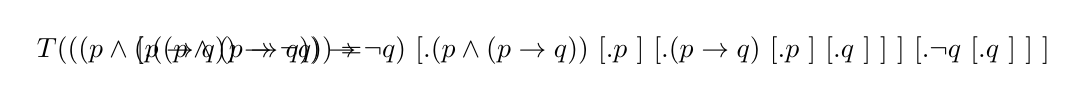
\begin{tikzpicture}
\node at (0,0) {$T(((p\land (p\to q)) \to \neg q))=$};
\node at (5,0) {\Tree [.$((p\land (p\to q))\to \neg q)$ [.$(p\land (p\to q))$ [.$p$ ] [.$(p\to q)$ [.$p$ ] [.$q$ ] ] ] [.$\neg q$ [.$q$ ] ] ]};

\end{tikzpicture}

Main operator: $\to$
\end{center}

		\item \
		
		\begin{center}
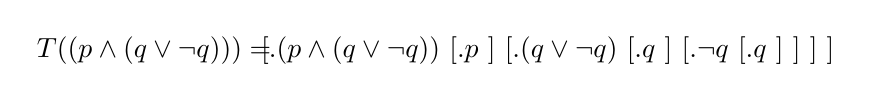
\begin{tikzpicture}
\node at (0,0) {$T((p\land (q\lor \neg q)))=$};
\node at (5,0) {\Tree [.$(p\land (q\lor \neg q))$ [.$p$ ] [.$(q\lor \neg q)$ [.$q$ ] [.$\neg q$ [.$q$ ] ] ] ]};

\end{tikzpicture}

Main operator: $\land$
\end{center}

		\item \
		
		\begin{center}
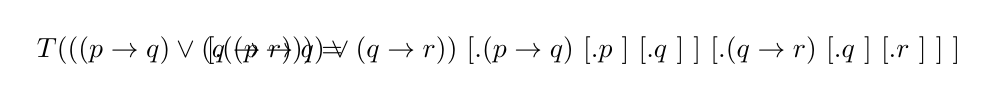
\begin{tikzpicture}
\node at (0,1) {$T(((p\to q)\lor (q\to r)))=$};
\node at (5,1) {\Tree [.$((p\to q)\lor (q\to r))$ [.$(p\to q)$ [.$p$ ] [.$q$ ] ] [.$(q\to r)$ [.$q$ ] [.$r$ ] ] ] };

\end{tikzpicture}

Main operator: $\lor$
\end{center}

			
		\item \
			 
			\begin{center}
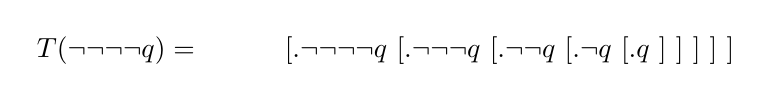
\begin{tikzpicture}
\node at (0,1) {$T(\neg\neg\neg\neg q)=$};
\node at (5,1) {\Tree [.$\neg\neg\neg\neg q$ [.$\neg\neg\neg q$ [.$\neg\neg q$ [.$\neg q$ [.$q$ ] ] ] ] ]};

\end{tikzpicture}

Main operator: $\neg$
\end{center}

In each of these cases, you can read the tree from bottom to top to get a construction of the formula in question from the sentence letters. This is the precise sense in which a parsing tree tracks the construction of a formula.
		
		
		\end{enumerate}
		
	\emph{The following point is the most difficult in this chapter. If you don't get it immediately, don't despair! Follow the advice on reading math: try to think this through, consider examples, draw pictures, etc. And then move on. The details of this proof are not the most important thing to take out of this chapter---the content of the main theorem is!}
		
	\item We will now prove that our recursive definition of $T$ indeed assigns to each formula $\phi$ a unique parsing tree, i.e. we prove that $T$ is a function. We do this in two steps, by proving two central lemmas. In order to properly state these lemmas, we need to read (i) and (ii) from (4.3.5) as \emph{conditions} on something being a tree for a formula---otherwise, we'd already assume the truth of these lemmas. The idea is that, for example, (4.3.5.i) says that a tree $T$ is a parsing tree of $p$ iff $T=p$. And (4.3.5.ii.a) says that $T$ is a parsing tree for $\neg\phi$ iff $T$ is of the form 
	\begin{center}
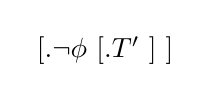
\begin{tikzpicture}
\node at (0,0) {\Tree [.$\neg \phi$ [.$T'$ ] ]};
\end{tikzpicture}
\end{center}
where $T'$ is a parsing tree for $\phi$. Similarly for (4.3.5.ii.b). With this understanding in mind, we can prove the following two lemmas:

		\begin{lemma}[Existence Lemma]
		For each $\phi\in\mathcal{L}$, $T(\phi)$ exists, i.e. there exists a tree that satisfies the conditions (i--ii) from (4.3.5).
		\end{lemma}
		\begin{proof}
		We prove the claim using induction.
		
			\begin{enumerate}[(i)]
			
				\item \emph{Base case}. Let $p\in\mathcal{P}$ be a sentence letter. By (4.3.5.i), $T(p)=p$. And, indeed, $p$ is a tree with $p$ as its only node. Hence, the base case holds.
				
				\item \emph{Induction steps}.
				
					\begin{enumerate}[(a)]
					
						\item Suppose the induction hypothesis that $T(\phi)$ exists. We need to show that $T(\neg \phi)$ exists. By (4.3.5.ii.a), we have that: 
						
						\begin{center}
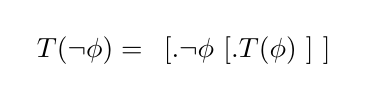
\begin{tikzpicture}
\node at (0,1) {$T(\neg \phi)=$};
\node at (2,1) {\Tree [.$\neg \phi$ [.$T(\phi)$ ] ]};
\end{tikzpicture}
\end{center}
But by the induction hypothesis $T(\phi)$ exists. But if $T(\phi)$ is a tree, so is $T(\neg\phi)$.

				\item Suppose the induction hypotheses that $T(\phi)$ and $T(\psi)$ exist. We need to show that $T((\phi\circ\psi))$ exists for $\circ=\land,\lor,\to,\leftrightarrow$. By (4.3.5.ii.b), we have that: 
						
						\begin{center}
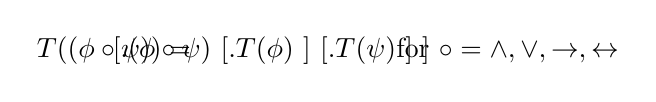
\begin{tikzpicture}
\node at (0,1) {$T((\phi\circ\psi))=$};
\node at (2,1) {\Tree [.$(\phi\circ\psi)$ [.$T(\phi)$ ] [.$T(\psi)$ ] ]};
\node at (5,1) {for $\circ=\land,\lor,\to,\leftrightarrow$};
\end{tikzpicture}
\end{center}
But by the induction hypothesis $T(\phi)$ and $T(\psi)$ both exist. But if $T(\phi)$ is a tree and $T(\psi)$ is a tree, so is $T((\phi\circ\psi))$.					
					\end{enumerate}
			
			\end{enumerate}
			
		Using induction on formulas, we conclude that for each $\phi\in\mathcal{L}$, $T(\phi)$ exists.
		\end{proof}
	\begin{lemma}[Uniqueness Lemma]
	Let $\phi\in\mathcal{L}$. Then $T(\phi)$ is unique, i.e. if $T_1(\phi)$ and $T_2(\phi)$ are two trees that satisfy the conditions (i--ii) from (4.3.5), then $T_1(\phi)=T_2(\phi)$.
	\end{lemma}
	
	\begin{proof}
	We prove this, once more, using induction.
		
			\begin{enumerate}[(i)]
			
				\item \emph{Base case}. Let $p\in\mathcal{P}$ be a sentence letter, and $T_1(p)$ and $T_2(p)$ two trees satisfying the  conditions (i--ii) from (4.3.5). But condition (4.3.5.i) says that $T(p)=p$, so $T_1(p)=p=T_2(p)$, which is what we needed to show.
								
				\item \emph{Induction steps}.
				
					\begin{enumerate}[(a)]
					
					\item Suppose the induction hypothesis that if $T_1(\phi)$ and $T_2(\phi)$ are two trees for $\phi$ which satisfy  conditions (i--ii) from (4.3.5), then $T_1(\phi)=T_2(\phi)$. Now consider two trees for $\neg \phi$, i.e. $T_1(\neg\phi)$ and $T_2(\neg \phi)$. By (4.3.5.ii.a), we have that:	
			\begin{center}
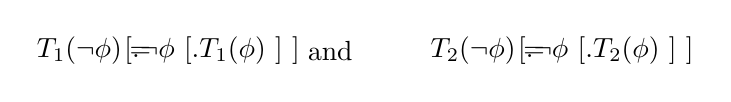
\begin{tikzpicture}
\node at (0,1) {$T_1(\neg \phi)=$};
\node at (1.5,1) {\Tree [.$\neg \phi$ [.$T_1(\phi)$ ] ]};
\node at (3,1) { and};
\node at (5,1) {$T_2(\neg \phi)=$};
\node at (6.5,1) {\Tree [.$\neg \phi$ [.$T_2(\phi)$ ] ]};
\end{tikzpicture}
\end{center}
where $T_1(\phi)$ and $T_2(\phi)$ are trees for $\phi$ which satisfy the conditions  (i--ii) from (4.3.5). But then, by the induction hypothesis, $T_1(\phi)=T_2(\phi)$. And so, $T_1(\neg\phi)=T_2(\neg \phi),$ as desired.

					
						\item Suppose the first induction hypothesis that if $T_1(\phi)$ and $T_2(\phi)$ are two trees for $\phi$ which satisfy  conditions (i--ii) from (4.3.5), then $T_1(\phi)=T_2(\phi)$. And suppose further that if $T_1(\psi)$ and $T_2(\psi)$ are two trees for $\psi$ which satisfy  conditions (i--ii) from (4.3.5), then $T_1(\psi)=T_2(\psi)$.
						
						Now consider two trees for $(\phi\circ\psi)$, for $\circ=\land,\lor,\to,\leftrightarrow$, $T_1((\phi\circ\psi))$ and $T_2((\phi\circ\psi))$. By (4.3.5.ii.a), we have that:	
			\begin{center}
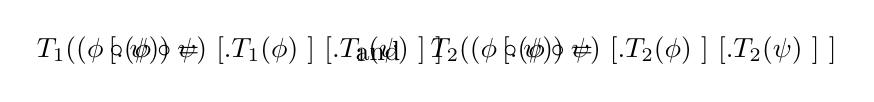
\begin{tikzpicture}
\node at (0,1) {$T_1((\phi\circ\psi))=$};
\node at (2,1) {\Tree [.$(\phi\circ\psi)$ [.$T_1(\phi)$ ] [.$T_1(\psi)$ ] ]};
\node at (3.3,1) { and};
\node at (5,1) {$T_2((\phi\circ\psi))=$};
\node at (7,1) {\Tree [.$(\phi\circ\psi)$ [.$T_2(\phi)$ ] [.$T_2(\psi)$ ] ]};
\end{tikzpicture}
\end{center}
where $T_1(\phi)$ and $T_2(\phi)$ are trees for $\phi$ which satisfy the conditions  (i--ii) from (4.3.5), and $T_1(\psi)$ and $T_2(\psi)$ are trees for $\psi$ which satisfy the conditions  (i--ii) from (4.3.5). But then, by the induction hypotheses, $T_1(\phi)=T_2(\phi)$ and $T_1(\psi)=T_2(\psi)$. And so, $T_1((\phi\circ\psi))=T_2((\phi\circ\psi)),$ as desired.

	\end{enumerate}
	
	\end{enumerate}
	
We conclude by using (i) and (ii) to infer by induction that the parsing tree for every formula is unique.
	
\end{proof}
	
	Put together, the two lemmas yield our unique readability theorem:
	\begin{theorem}
	For each formula $\phi\in\mathcal{L}$ there exists a unique parsing tree, $T(\phi)$ as defined by (4.3.5).
	\end{theorem}
	
	This theorem is of fundamental importance for what we're doing in propositional logic. Essentially, it guarantees that we can use function recursion on $\mathcal{L}$. Why? Because the theorem tells us that we can calculate a recursively defined function on $\mathcal{L}$ following the formulas parsing tree---\emph{and this is the only way in which the function can be calculated}. In fact, this theorem guarantees that propositional logic can be computer implemented---a computer can construct the parsing tree for a formula in order to ``understand'' it.
	
	\item We'll conclude the section by discussing an \emph{algorithm} for determining whether a given expression $\sigma$ is a formula. First, let's clarify what we understand under the term ``algorithm.'' In mathematics, an algorithm is typically understood as a finite set of precise instructions which, if followed, are supposed to complete a specific task. Hence an algorithm itself is not a computer program but the procedure that underlies the computer program. We can thus describe an algorithm in natural language without focusing on a specific \emph{implementation} of the algorithm in a programming language. 
	
	\item The task that our algorithm is supposed to fulfill is to determine whether a given expression is a formula. We hereby assume that the expression is formed entirely out of symbols from the alphabet, since by 4.2.5, if it's not, we can already exclude that it's a formula. Here is our algorithm:
	\begin{enumerate}[1.]
			
				\item Write down the expression $\sigma$ and look at it. Proceed to step 2.
				
				\item Does the expression you're currently looking at contain the same number of $($'s and $)$'s?
				\begin{enumerate}[(a)]
				
					\item If not, terminate: $\sigma$ is not a formula!
					
					\item If yes, proceed to step 3.
				
				\end{enumerate}
				
				\item Is the expression you're currently looking at of the form $p$?
				
				\begin{enumerate}[(a)]
				
					\item If not, proceed to step 4.
				
					\item If yes, write a $\checkmark$ next to it and proceed to step 6.
					
				\end{enumerate}
				
				\item Is the expression you're currently looking at of the form $\neg \tau$?

				\begin{enumerate}[(a)]
				
					\item If not, proceed to step 5.

					
					\item If yes, apply the following rule:
					\begin{center}
					\Tree [.$\neg \tau\checkmark$ [.$\tau$ ] ]
					\end{center}
					Then proceed to step 6.
										
				
				\end{enumerate}
											
	
			\item Is the expression you're currently looking at of the form $(\tau\circ\pi)$, $\circ=\land,\lor,\to,\leftrightarrow$,  and there is no other connective $\square=\land,\lor,\to,\leftrightarrow$ such that the expression is of the form $(\tau'\square\pi')$ and $\square$ is enclosed in fewer parentheses than $\circ$?				
	
			\begin{enumerate}[(a)]
		
				\item If not, terminate: $\sigma$ is not a formula!
				
				\item If yes, apply the following rule:
			
				\begin{center}
				\Tree [.$(\tau\circ\pi)\checkmark$ [.$\tau$ ] [.$\pi$ ] ]
				\end{center}
			
				Then proceed to step 6.	
			
			\end{enumerate}
		
			\item In the tree you've constructed so far, is there an expression at a leaf without a $\checkmark$ next to it?
		
			\begin{enumerate}[(a)]
			
				\item If no, terminate: $\sigma$ is a formula \smiley		
				
				\item If yes, then pick one and look at it. Go back to step 2.
			
		
			\end{enumerate}
	
		\end{enumerate}
		
	\item We will not prove that this algorithm actually completes its task, we won't \emph{formally verify} the algorithm. To do so, is actually not that hard given all the facts we've already observed. But it's tedious and so we'll leave the task to the interested reader. Note that what you would need to show are three things: (i) the algorithm always terminates, (ii) if the algorithm terminates and says that the expression is a formula, then it is indeed a formula, and (iii) if the algorithm terminates and says that the expression is not a formula, then it is indeed not a formula. Here we simply observe (again without proof) that the algorithm, if applied to a formula, actually yields the parsing tree of that formula. To see this, try it out! Apply the algorithm to some formulas and see what you get. Here we give just one example:
	\begin{center}
	\Tree[.$(p\lor (q\lor (r\leftrightarrow (\neg s\land t))))\checkmark^{5.b}$ [.{$p\checkmark^{3.b}$} ] [.{$(q\lor (r\leftrightarrow (\neg s\land t)))\checkmark^{5.b}$} [.{$q\checkmark^{3.b}$} ] [.{$(r\leftrightarrow (\neg s\land t))\checkmark^{5.b}$} [.$r\checkmark^{3.b}$ ] [.$(\neg s\land t)\checkmark^{5.b}$ [.$\neg s\checkmark^{4.b}$ [.$s\checkmark^{3.b}$ ] ] [.$t\checkmark^{3.b}$ ] ] ] ] ]
	
	\emph{Note that in the first step (5.b), we parse according to the first $\lor$ because it's in fewer parentheses than the second $\lor$, the $\leftrightarrow$ and the $\land$.}
	\end{center}
	So, effectively, what the algorithm does is what a computer would do (described on a very abstract level) if given an expression and asked whether it makes sense in propositional logic.
	
	\item We conclude the section with two example applications of the algorithm to illustrate how it can be used to show that something \emph{isn't} a formula:
	
		\begin{enumerate}[(i)]
		
			\item \emph{Claim}. $((p\land q)\to (r))\notin\mathcal{L}$
			
			\item[] \emph{Algorithmic proof}.

			\begin{center}		
				\Tree [.$((p\land q)\to \neg(r))\checkmark^{5.b}$ [.$(p\land q)\checkmark^{5.b}$ [.$p\checkmark^{3.b}$ ] [.$q\checkmark^{3.b}$ ] ] [.$\neg(r)\checkmark^{4.b}$ [.$(r)\frownie^{5.a}$ ] ] ] 
			\end{center}
			
			\item \emph{Claim}. $\neg\neg(p(\leftrightarrow) q)\notin\mathcal{L}$.
			
			\item[] \emph{Algorithmic proof}.
			
				\begin{center}
				\Tree [.${\neg\neg(p(\leftrightarrow) q)}\checkmark^{4.b}$ [.${\neg(p(\leftrightarrow) q)}\checkmark^{4.b}$ [.${(p(\leftrightarrow) q)}\checkmark^{5.b}$ [.$(p(\frownie^{2.a}$ ] [.$)q)\frownie^{2.a}$ ] ] ] ]
				\end{center}
		\end{enumerate}
	
	\end{enumerate}
	
	
\section{Function Recursion on Propositional Languages}

	\begin{enumerate}[\thesection.1]

		\item In the previous section, we've given a justification for using function recursion on $\mathcal{L}$. Now, we'll define two important syntactic functions, i.e. functions with domain $\mathcal{L}$. The importance of these functions derives from their wide-spread use in logical literature (way beyond propositional logic). But also in our course, they will play an important role here and there.
		
	  \item The first of the two functions, we'll define a function that maps each formula to the set of formulas it was constructed from.
		These formulas are called the \emph{sub-formulas} of the formula in question.
		We define the function as follows using function recursion:
		\begin{enumerate}[(i)]
		  \item%
			$sub(p)=\{p\}$ for $p\in\mathcal{P}$
		  \item%
			\begin{enumerate}[(a)]
			  \item%
				$sub(\neg\phi)= sub(\phi)\cup\{\neg \phi\}$
			  \item%
				$sub((\phi\circ\psi))= sub(\phi)\cup sub(\psi)\cup\{(\phi\circ\psi)\}$
			\end{enumerate}
		\end{enumerate}
		Let's consider two examples.
		We have:
		\begin{itemize}
		  \item%
			$sub(\neg \neg p)=\{p,\neg p, \neg\neg p\}$
		  \item%
			$sub(((p\land q)\lor r))=\{p,q,r,(p\land q), ((p\land q)\lor r)\}$
		\end{itemize}
		In order to understand this definition,
		follow the advice for understanding a definition from lecture 2!

	\item One thing that might help us understanding sub-formulas better is to compare them to notions we've previously introduced. For this purpose, we'll prove the following proposition:
	
		\begin{proposition}
		Let $\phi\in\mathcal{L}$ be a formula. Then the elements of $sub(\phi)$ are precisely the formulas that occur in $T(\phi)$.
		\end{proposition}
		\begin{proof}
		We prove this fact using---surprise---induction.
		
		\begin{enumerate}[(i)]
		
			\item \emph{Base case}. Let $p\in\mathcal{P}$ be a sentence letter. Then $sub(p)=\{p\}$ and $T(p)=p$. Hence $sub(p)$ is precisely the set of formulas that occur in $T(p)$.
			
			\item \emph{Induction steps}. 
				\begin{enumerate}[(a)]

					\item Assume the induction hypothesis that $sub(\phi)$ are precisely the formulas that occur in $T(\phi)$. Now consider $\neg \phi$. We know by definition of $sub$, that $sub(\neg\phi)=sub(\phi)\cup\{\neg\phi\}$. By the (ii.a) definition of parsing trees, we know furthermore that:
					\begin{center}
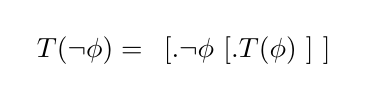
\begin{tikzpicture}
\node at (0,0) {$T(\neg \phi)=$};
\node at (2,0) {\Tree [.$\neg \phi$ [.$T(\phi)$ ] ]};
\end{tikzpicture}
\end{center}
Hence the formulas that occur in $T(\neg\phi)$ are precisely the formulas that occur in $T(\phi)$ plus the formula $\neg\phi$. But this is just another way of saying that the formulas in $T(\neg\phi)$ are  $sub(\phi)\cup\{\neg\phi\}=sub(\neg\phi),$ as desired.

			\item Assume the induction hypotheses that $sub(\phi)$ are precisely the formulas that occur in $T(\phi)$ and $sub(\psi)$ are precisely the formulas ocuring in $T(\psi)$. Now consider $(\phi\circ\psi)$, for $\circ=\land,\lor,\to,\leftrightarrow$. We know by definition of $sub$, that $sub((\phi\circ\psi))=sub(\phi)\cup sub(\psi)\cup\{(\phi\circ\psi)\}$. By the (ii.a) definition of parsing trees, we know furthermore that:
					\begin{center}
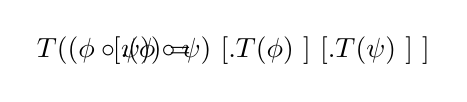
\begin{tikzpicture}
\node at (0,0) {$T((\phi\circ\psi))=$};
\node at (2,0) {\Tree [.$(\phi\circ\psi)$ [.$T(\phi)$ ] [.$T(\psi)$ ] ]};
\end{tikzpicture}
\end{center}
Hence the formulas that occur in $T((\phi\circ\psi))$ are precisely the formulas that occur in $T(\phi)$, plus the formulas in $T(\psi)$, plus $(\phi\circ\psi)$. But this is just another way of saying that the formulas in $T((\phi\circ\psi))$ are $sub(\phi)\cup sub(\psi)\cup\{(\phi\circ\psi)\}=sub((\phi\circ\psi)),$ as desiderd.

				\end{enumerate}
		
		\end{enumerate}
		We can thus use induction to infer that the claim holds for all $\phi$.		
		\end{proof}

	\item We move to the second important syntactic function, the so-called measure of \emph{complexity}. In order to define this function, we make use of the maximum function $max:\mathbb{N}^2\to\mathbb{N}$, which is defined as follows:
	\[max(n,m)=\begin{cases} n &\text{if }n>m\\ m &\text{if }m>n\\n& \text{if }n=m\end{cases}\] So, we get, for example, $max(2,3)=3, max(3,2)=3, max(2,2)=2$, and so on. Using $max$, the (recursive) definition of the complexity function $c:\mathcal{L}\to\mathbb{N}$ is as follows:
	\begin{enumerate}[(i)]
	
		\item $c(p)=0$ for $p\in\mathcal{P}$
		
		\item \begin{enumerate}[(a)]
		
			\item $c(\neg\phi)=c(\phi)+1$
			
			\item $c((\phi\circ\psi))=max(c(\phi), c(\psi))+1$, for $\circ=\land,\lor,\to,\leftrightarrow$.
		
		\end{enumerate}
	
	\end{enumerate}
Let's consider some examples. We have:
	\begin{itemize}
	
		\item $c(\neg p)=1$, $c((p\land q))=1, c((p\lor q)=1, \mathellipsis$
		
		\item $c(\neg\neg p)=2$, $c(\neg (p\land q))=2$, $c((\neg p\land \neg q))=2, \mathellipsis$
	
	\end{itemize}
	
	Can we somehow narrow down what $c$ precisely measures? Think about it before you read the next point. 

	\item We will now prove a proposition that gives us an intuitive reading of the function $c$:
	
	\begin{proposition}
	Let $\phi\in\mathcal{L}$ be a formula. Then $c(\phi)$ is the length of the longest path in $T(\phi)$ which starts from the root (counted in number of edges travelled). In other words, $c(\phi)$ gives us the \emph{height} of the parsing tree $T(\phi)$.
	\end{proposition}
	\begin{proof}
	How are we going to prove this? You know it!
	
\begin{enumerate}[(i)]
		
			\item \emph{Base case}. Let $p\in\mathcal{P}$ be a sentence letter. Then $T(p)=p$. But the only path you can travel from the root in $p$ is the trivial path of length zero, which just stops immediately at $p$. Since $c(p)=0$, this just means that the base case holds.
			
			\item \emph{Induction steps}. 
				\begin{enumerate}[(a)]

					\item Assume the induction hypothesis that $c(\phi)$ is the length of the longest path from the root in $T(\phi)$. Now consider $\neg \phi$. By the (ii.a) definition of parsing trees, we know that:
					\begin{center}
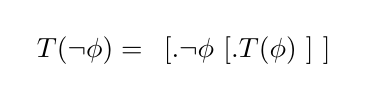
\begin{tikzpicture}
\node at (0,0) {$T(\neg \phi)=$};
\node at (2,0) {\Tree [.$\neg \phi$ [.$T(\phi)$ ] ]};
\end{tikzpicture}
\end{center}
Now think about the longest path you can travel from the root in $T(\neg\phi)$. Well, it's going to be the longest path you can travel in $T(\phi)$ plus one edge to the new root, i.e. $\neg\phi$. Since $c(\neg\phi)=c(\phi)+1$, this means that, by the induction hypothesis, the claim holds.

			\item Assume the induction hypotheses that $c(\phi)$ is the length of the longest path from the root in $T(\phi)$ and $c(\psi)$ is the length of the longest path from the root in $T(\psi)$. By the (ii.a) definition of parsing trees, we know that:
					\begin{center}
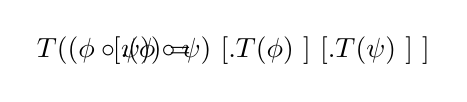
\begin{tikzpicture}
\node at (0,0) {$T((\phi\circ\psi))=$};
\node at (2,0) {\Tree [.$(\phi\circ\psi)$ [.$T(\phi)$ ] [.$T(\psi)$ ] ]};
\end{tikzpicture}
\end{center}
Now think about the longest path you can travel in $T((\phi\circ\psi))$. Well, take the longest path you can find in either $T(\phi)$ or $T(\psi)$. Let's suppose that the path is in $T(\phi)$ (if it is in $T(\psi)$, the argument is completely analogous). The longest path you can travel from the root in $T((\phi\circ\psi))$ is going to be precisely this path plus the one new edge connecting $T(\phi)$ to the new root $(\phi\circ\psi)$. Since $c((\phi\circ\psi))=max(c(\phi),c(\psi))+1$, this just means that the claim also holds here. 
				\end{enumerate}
		
		\end{enumerate}
		We can thus use induction to infer that the claim holds for all $\phi$.			
	\end{proof}
	
	\item This completes our discussion of function recursion on $\mathcal{L}$ by means examples. In order to get a real good grip on how the method works, it's best for you to try your hand at it, i.e. try to define your own syntactic functions using function recursion. Among the exercises, you can find some functions you can try to define.

	\end{enumerate}

\section{Some Useful Notational Conventions}

	\begin{enumerate}[\thesection.1]

		\item So far, we've been very precise about our use of parentheses. And for good reason: as we discussed in \S4.3, our tidy use of parentheses is what guaranteed unique readability. But, at the same time, writing all of these parentheses can be exhausting. And, as I said in the lecture, logicians are lazy: they don't like to do unnecessary things. So, over the years, some generally agreed upon conventions have emerged for leaving out parentheses, which we'll briefly discuss in this section.
		
		\item Before we begin, note that conventional notation is only ever allowed outside the context of syntax theory, i.e. in semantics and proof theory. And even there, it's often better to be safe than sorry. As we said a couple of times by now: the parentheses are there for a reason. It's much easier to make mistakes using conventional notation than it is in official notation. That being said, conventional notation can be a real boon on your wrist.
		
		\item The first convention is that you can always omit any outermost parentheses. So, instead of $(p\land q)$, you can simply write $p\land q$. The reasoning behind this is that these are easy to fill in: if a logician writes $p\lor q$, it's pretty clear what they mean: $(p\lor q$).
		
		\item The second convention is that in a series of $\lor$'s or $\land$'s, you can leave out the repeatedly nested parentheses. So, for example, instead of the official $((p\land (q\land (r\land (s\land t)))))$, we can simply write $p\land q\land r\land s\land t$ (also applying the convention about outermost parentheses). Note that this convention really introduces some ambiguity into our language. The conventional formula $p\lor q\lor r$ has indeed two ways of being parsed:
		\begin{center}
		
		\begin{tabular}{c c c}
		\begin{tikzpicture}
		{\Tree [.$p\lor q\lor r$ [.$p$ ] [.$q\lor r$ [.$q$ ] [.$r$ ] ] ]}
		\end{tikzpicture}

		& 
		
		\qquad \raisebox{7.5ex}{vs.} \qquad 
				\begin{tikzpicture}

		{\Tree [.$p\lor q\lor r$ [.$p\lor q$ [.$p$ ] [.$q$ ] ] [.$r$ ] ]}
		\end{tikzpicture}

		\end{tabular}
		\end{center}
This makes the convention a bit harder to justify. But note that the two different ``readings'' of the formula don't really say anything different. Take the following two sentences: 
	\begin{itemize}

		\item I have toast, or I have eggs or pancakes
		
		\item I have toast or eggs, or I have pancakes

	\end{itemize}
They really seem to say the same thing. We'll only be able to properly justify the convention in the next chapter, when we talk about logical equivalence, but for now, I hope these examples illustrate why we can allow for this little bit of ambiguity. Note that in \emph{mixed} series of $\land$ and $\lor$, we \emph{cannot} omit parentheses. I.e. $p\land (q\lor r)$ needs to stay just that.

		\item Finally, the most complicated convention concerns the interaction of the connectives. The idea is that if we agree upon which connective we should read first, we can drop a bunch of parentheses. For example, if we say that we always read $\to$ before $\land$ if there's an ambiguity, then the previously ambiguous expression $p\land q\to r$, with the two readings
				\begin{center}
		
		\begin{tabular}{c c c}
		\begin{tikzpicture}
		{\Tree [.$p\land q\to r$ [.$p$ ] [.$q\to r$ [.$q$ ] [.$r$ ] ] ]}
		\end{tikzpicture}

		& 
		
		\qquad \raisebox{7.5ex}{vs.} \qquad 
				\begin{tikzpicture}

		{\Tree [.$p\land q\to r$ [.$p\land q$ [.$p$ ] [.$q$ ] ] [.$r$ ] ]}
		\end{tikzpicture}

		\end{tabular}
		\end{center}
now unambiguously, gets the second of the two readings. That is, $p\land q\to r$ is then simply read as $(p\land q)\to r$. This is the idea of \emph{binding strength}: we say that $\land$ \emph{binds stronger} than $\to$. This idea allows us to leave out a bunch of parentheses, which we can easily fill in by reading the right operator first. 

	\item The relative binding strength of the operators is given in the following diagram:
\[{\neg}>{\land}={\lor}>{\to}>{\leftrightarrow}.\] Explicitly, this means that, in a case of conflict, you always read the $\leftrightarrow$ first, then $\to$, then $\lor$ and $\land$, and only finally $\neg$. Note that $\land$ and $\lor$ have precisely the same binding strength, so in expressions like $p\land (q\lor r)$, we really can't leave out any parentheses. But if we consider an expression like $((p\land q)\leftrightarrow (p\leftrightarrow q))$, we can easily leave out a some:
	\begin{itemize}
	
		\item According to the first convention, we can leave out the outermost parentheses, yielding $(p\land q)\leftrightarrow (p\leftrightarrow q)$.
		
		\item Now, since we know that we'll always parse according to $\leftrightarrow$ before $\land$, this means that we can leave out the parentheses around the $\land$, giving us $p\land q\leftrightarrow (p\leftrightarrow q)$.
		
		\item Can we also leave out the last pair of parentheses? ---No! For in $p\land q\leftrightarrow p\leftrightarrow q$, there would be a conflict between two readings:
	\begin{center}
		
		\begin{tabular}{c c c}
		\begin{tikzpicture}
		{\Tree [.$p\land q\leftrightarrow p\leftrightarrow q$ [.$p\land q$ [.$p$ ] [.$q$ ] ] [.$p\leftrightarrow q$ [.$p$ ] [.$q$ ] ] ]}
		\end{tikzpicture}

		& 
		
		\qquad \raisebox{7.5ex}{vs.} \qquad & 
				\begin{tikzpicture}
		{\Tree [.$p\land q\leftrightarrow p\leftrightarrow q$ [.$p\land q\leftrightarrow p$ [.$p\land q$ [.$p$ ] [.$q$ ] ] [.$p$ ] ] [.$q$ ] ]}
		\end{tikzpicture}

		\end{tabular}
		\end{center}
		
		\item So, the best we can do is $p\land q\leftrightarrow (p\leftrightarrow q)$.
	
	\end{itemize}
	
	\item These ideas need some getting used to. For that reason, there are plenty of exercises included at the end of this section (4.8.9 and 4.8.10), solutions for which can be found in the appendix.
	
	\item We conclude with a last remark about conventional notation. You might wonder: Well, these are pretty clear conventions. Surely, a computer can learn them. Why can't we devise an official definition that has unique readability and respects these conventions? ---And you would be right! This \emph{is} possible. It's just not very practical for most purposes. The official definition of a formula would thereby become much more complicated. This would have the consequence that proofs by induction and function recursion would become horribly complicated to carry out, too. Additionally, if we care about efficiency (as we often do with computers), it turns out to be way more efficient to use our official definition and to translate between official and conventional notation that to carry out everything in conventional notation. And you can essentially see why: because \emph{every} recursive definition would become more complicated---and we need \emph{a lot} of them. So, we'll stick to our official notation for official purposes and use conventional notation for fun. 

	\end{enumerate}

\section{Core Ideas}

\begin{itemize}

	\item A formal language is defined by a vocabulary (symbols) and a grammar (rules for well-formed expressions).
	
	\item The vocabulary of a propositional language consists of a set of sentence letters $\mathcal{P}$, the sentential connectives $\neg,\land,\lor,\to,\leftrightarrow$, and the parentheses $($ and $)$.
	
	\item The set $\mathcal{L}$ of formulas is inductively defined as the smallest set containing the sentence letters and which is closed under the sentential connectives. 
	
	\item Formalization is the process of abstracting ordinary language expressions into a propositional language. \emph{Use the guidelines}.
	
	\item Syntactic recursion works by specifying the value for the sentence letters and how to calculate the value for a complex formula from the values for its subformulas.
	
	\item The parsing tree of a formula gives you its internal structure: it shows how the formula was constructed.
	
	\item The unique readability theorem guarantees that syntactic recursion works and that formulas are computer readable. It states that every formula has a unique parsing tree.
	
	\item There is a useful algorithm for checking whether an expression is a formula.
	
	\item Outside of syntax theory, the notational conventions are useful. But use them with caution.

\end{itemize}

\section{Self Study Questions}

	\begin{enumerate}[\thesection.1]

		\item Suppose that an expression contains absolutely no parentheses. What is the best we can say about the expression?
		
			\begin{enumerate}[(a)]

				\item The expression is not a formula.
				
				\item If the expression is a formula, then it is a sentence letter.
				
				\item If the expression is a formula, then it cannot contain $\land,\lor,\to,\leftrightarrow$.
				
				\item There is an even number of negations in the expression.
	
			\end{enumerate}
			
		\item You're asked to determine whether an expression is a formula. In which order would you apply the following techniques?
		
		\begin{enumerate}[(a)]
		
			\item Try to prove it definitionally (as in 4.1.9)
		
			\item Check whether the expression contains symbols not from the vocabulary (using Proposition 4.2.5).
			
			\item Apply the algorithm (4.3.10).
			
			\item Check whether the expression contains as many $($'s as $)$'s (using the solution to exercise (4.8.8)).
		
		\end{enumerate}
		
	\item Can you always see whether a formula is written in conventional notation?
	
	\begin{enumerate}[(a)]
	
		\item Yes, I simply construct the parsing tree for the expression.
		
		\item No, because a formula written in notational convention does  not need to contain an even number of parentheses.
	
		\item Yes, you can apply the algorithm (4.3.10) for that.
	
		\item No, it needs to be clear from the context.
	
	\end{enumerate}
	
	\item A formula has complexity four. Which of the following can you infer from that?
		
		\begin{enumerate}[(a)]
		
			\item The formula contains at least four connectives.
			
			\item The formulas contains at most four connectives.
			
			\item The formula contains at most four negations.
			
			\item The parsing tree of the formula has at most four nodes.

			\item The parsing tree of the formula has exactly four nodes.
			
			\item The parsing tree of the formula has at least five nodes.
		
		\end{enumerate}

	\end{enumerate}
\section{Exercises}


	\begin{enumerate}[\thesection.1]
	
		\item $[h]$ Translate the following statements into a suitable propositional language! Don't forget the translation key.
			
			\begin{enumerate}

				\item Alan Turing built the first computer but Ada Lovelace invented the first computer algorithm.
			
				\item Only if Alan Turing built the first computer, it's Monday today.
			
				\item Either Alan Turing or Ada Lovelace is your favorite computer scientist.
			
				\item Today is Monday if and only if both yesterday was Tuesday and tomorrow is Saturday.
			
			\end{enumerate}

		\item $[h]$ Translate the following statements into English/Dutch. Use the following translation key: 
		
		\begin{center}
			\begin{tabular}{c c l}
		
			 $p$ & : & I'm happy/Ik ben blij\\[1ex]
			
			 $q$ & : & I clap my hands/Ik klap in mijn handen\\[1ex]
			
			 $r$ & : & You're happy/Jij bent blij\\[1ex]
			
			 $s$ & : & You clap your hands/Jij klapt in je handen\\[1ex]
			
			 $t$ & : & We both clap our hands/Wij klappen in onze handen
			 \end{tabular}
		
		\end{center}
		
		\begin{enumerate}[(a)]
		
			\item $\neg\neg (p\land q)$
		
			\item $(\neg p\to \neg q)$
			
			\item $(p\leftrightarrow (\neg r\land q))$
			
			\item $((q\land s)\to t)$
		
			\item $((q\land s)\to (p\lor r))$
			
			\item $(((p\land q)\lor (r\land s))\land \neg ((p\land q\land r\land s)))$
		
		\end{enumerate}
		
		\item Give an inductive definition of the set of all formulas of $\mathcal{L}$ that only contain $p,q,\neg,\land,(,$ and $)$.
		
		\item Use the algorithm from 4.3.10 to decide whether the following expressions are formulas:
		
		\begin{enumerate}[(a)]
		
			\item $(q\leftrightarrow (p\land (q\lor (r\land \neg s)))$
		
			
			\item $((p\land q)\lor (p\land (q\to\neg q)))$
			
			\item $(p\to (p\to ((p\land p)\leftrightarrow p\lor p)))$
			
			\item $\neg\neg (\neg\neg p\land (q\lor q) )$
			
		\end{enumerate}
		
		\item Use function recursion to define the following syntactic functions:
		
		\begin{enumerate}
		
			\item $[h]$ the function $\#_{conn}:\mathcal{L}\to\mathbb{N}$, which counts the number of sentential connectives in a formula $\phi$.
			
			\item the function $\#_(:\mathcal{L}\to\mathbb{N}$, which counts the number of left brackets in a formula $\phi$. 
			
			\item the function $\#_{\mathcal{P}}:\mathcal{L}\to\mathbb{N}$, which counts the number of sentence letters in a formula $\phi$.
			
			\item the function $\mathbf{1}_p:\mathcal{L}\to\{0,1\}$, which assigns one to a formula $\phi$ if $p\in sub(\phi)$ and zero otherwise.
		
		\end{enumerate}
		
		\item $[\nosym]$ Consider the following recursively defined functions on $\mathcal{L}$. What do they (in ordinary words) measure?
		
			\begin{enumerate}[(a)]
			
				\item $f:\mathcal{L}\to\mathbb{N}$ defined by:
				
					\begin{enumerate}[(i)]

					\item $f(p)=1,$ for $p\in\mathcal{P}$

					\item 			\begin{enumerate}[(a)]

					\item $f(\neg \phi)=f(\phi)+1,$

					\item $f((\phi\circ \psi))=f(\phi)+f(\psi)+3,$ for $\circ=\land,\lor,\to,\leftrightarrow.$
					
					\end{enumerate}
					\end{enumerate}
					
				\item $g:\mathcal{L}\to\mathbb{N}$ defined by:
				
					\begin{enumerate}[(i)]

					\item $g(p)=0,$ for $p\in\mathcal{P}$

					\item 			\begin{enumerate}[(a)]

					\item $g(\neg \phi)=g(\phi)+1,$

					\item $g((\phi\circ \psi))=g(\phi)+g(\psi),$ for $\circ=\land,\lor,\to,\leftrightarrow.$
					
					\end{enumerate}
					\end{enumerate}
					
					\item (this is a tricky one) $h:\mathcal{L}\to\{0,1\}$ defined by:
				
					\begin{enumerate}[(i)]

					\item $h(p)=1,$ for $p\in\mathcal{P}$

					\item 			\begin{enumerate}[(a)]

					\item $h(\neg \phi)=\begin{cases}
					0 &\text{if }h(\phi)=1\\
					1 & \text{if }h(\phi)=0
					\end{cases}$

					\item $h((\phi\circ \psi))=\begin{cases}
					1&\text{if }h(\phi)=1\text{ and }h(\psi)=1\\
					1&\text{if }h(\phi)=0\text{ and }h(\psi)=0\\
					0 & \text{otherwise}
					\end{cases}$ 
					
					\item[] for $\circ=\land,\lor,\to,\leftrightarrow.$
					
					\end{enumerate}
					\end{enumerate}
			
			\end{enumerate} 
		
		\item Use proof by induction to prove that the number of elements in $sub(\phi)$ is at most $2\cdot \#_{conn}(\phi)+1$.

		\item $[h]$ Prove (using induction on formulas) that for each formula $\phi\in\mathcal{L}$, the number of $($'s and the number of $)$'s is equal. Derive as a corollary a necessary condition for formula-hood and discuss why the condition is better than the one given in (4.2.4).
		
		\item Translate the following formulas written using the notational conventions into official notation:
		
		\begin{enumerate}[(a)]

		\item  $\neg p\land q$

		\item  $\neg(p\land q\to \neg p\lor\neg q)$
		
		\item  $p\lor p\leftrightarrow \neg p$

		\item  $(p\lor q)\land r$
		
		\item $p\to p\leftrightarrow p\to p$

		\item  $\neg p \land (q\lor r\to p\leftrightarrow q)$
		
		\item $p\land (p\lor q)$ 

		\item $p\to q\lor q\leftrightarrow r$

		\item $p\to q\leftrightarrow \neg q\to \neg p$  

		\item $\neg\neg\neg p$

		\item ${p} \to {p} \leftrightarrow {p}\lor \neg {p}$

		\item $p\lor q\to \neg r\land (s\leftrightarrow {p})$

		\end{enumerate}
		
	\item Take the following formulas and write them according to our notational conventions:
	
		\begin{enumerate}
		
			\item $(p\land q)$
		
			\item $\neg\neg q$
			
			\item $(p\land (r\lor q))$
			
			\item $(p\to (r\lor (p\land (q\leftrightarrow r))))$
			
			\item $(p\lor \neg (p\lor q))$
			
			\item $((p\land q)\to r)$
			
			\item $(((p\lor q)\to \neg q)\leftrightarrow r)$
			
			\item $((p\land q)\land r)$
			
			\item $(p\land (q\land r))$
			
			\item $(p\lor (q\lor r))$
			
			\item $(p\land (q\lor r))$
			
			\item $(p\land (q\to r))$
				
		\end{enumerate}
		
		\item (This is a real challenge, only try this is you have enough time and energy): Write an algorithm that translates a formula from conventional into official notation. 

	\end{enumerate}

\section{Further Readings}

We're starting to get into logic proper. Recommendations for further readings that I can give you at this point will be chapters from other logic books, which cover the same material but in slightly different way. Note, however, that if you look into another logic textbook, you will (most likely) encounter different ways of doing things. Here are just some examples of what I mean:
	\begin{itemize}
	
		\item Some authors use different terminology. For example, they may call sentence letters ``propositional variables'' or sentential connectives ``propositional connectives.''
		
		\item Some authors may have different definitions of formulas. It's possible, for example, to demand that also negations are enclosed by parentheses, so that $\neg p$ is not a formula only $(\neg p)$ is.
	
		\item Some authors use different symbols for the connectives, such as $\supset$ instead of our $\to$ or $\equiv$ instead of our $\leftrightarrow$. 
		
		\item Some authors use $A,B,C,\mathellipsis$ for formulas, rather than our $\phi,\psi,\theta,\mathellipsis.$
		
		\item Some authors might use proof by induction in a different (but equivalent) way. For example, they might use mathematical induction on the complexity of formulas instead of our method, which is known in the literature as \emph{structural} induction.
		
		\item Some authors may use terminology in a slightly different way. For example, complexity is sometimes defined so that it doesn't correspond to the height of the parsing tree but rather the number of logical connectives in the formula. 
		
		\item They might prove different theorems or the same theorems in different ways.
	
	\end{itemize}
	
These are really just some of the possible differences you may encounter. If you continue with my literature recommendations, you have to brace yourself for that. But there are also some reasons for why it's a good idea to look at other texts despite these potential obstacles:
	\begin{itemize}
	
		\item Regardless of these differences, the books that I'm recommending are dealing with the same subject matter---just in a slightly different way. And this different perspective might help you understand better what's going on.
		
		\item When you continue your studies, you will see that there are  many, many different notations or, more generally, ways of doing things around. This equally applies in logic, mathematics, computer science, and other related disciplines. The earlier you get used to the plurality, the better.
			
		\item Other textbooks are a great source of additional exercises (though typically without solutions, as I mentioned in the lecture).	
			
	\end{itemize}
So, here are my recommendations for book-chapters that deal with the same material in comparable ways. 

	\begin{itemize}
	
		\item Section 2.1 of Dalen, Dirk van. 2013. \emph{Logic and Structure}. 5$^\text{th}$ edition. London, UK: Springer.
		
		\item Sections 1.0, 1.1 and 1.3 of Enderton, Herbert. 2001. \emph{A Mathematical Introduction to Logic}. 2$^\text{nd}$ edition. San Diego, CA: Harcourt/Academic Press.
		
		\item The reader \emph{Parvulae Logicales INDUCTIE} by Albert Visser, Piet Lemmens, and Vincent van Oostrom from the 2015 installment of the course. You can find this on blackboard.
	
	\end{itemize}
One last thing: don't buy these books until you really feel like the book will help you a lot. Look at them in the library first (or online, if possible)!


\vfill

\hfill \rotatebox[origin=c]{180}{
\fbox{
\begin{minipage}{0.5\linewidth}

\subsection*{Self Study Solutions}

\emph{Some explanations in the appendix.}

\begin{enumerate}

	\item[4.7.1] (c)
	
	\item[4.7.2]  first (b), then (d), then (c), then (a)
	
	\item[4.7.3] (d) 
	
	\item[4.7.4] (a), (f)
		
\end{enumerate}


\end{minipage}}}

%%% Local Variables: 
%%% mode: latex
%%% TeX-master: "../../logic.tex"
%%% End:
